\documentclass[tikz]{standalone}
\usepackage{lmodern}
\usetikzlibrary{shadows,chains,scopes}
\usetikzlibrary{decorations.pathmorphing, shapes}
\begin{document}
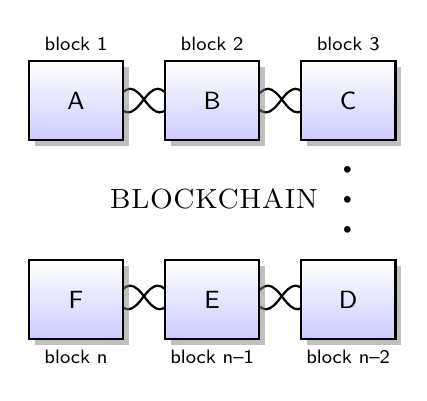
\begin{tikzpicture}
  [
    start chain=going right,
    node distance=5mm,
    every on chain/.style={
      thick,
      draw=black,
      top color=white,
      bottom color=blue!20,
      font=\sffamily\small,
      minimum width=12mm,
      minimum height=10mm,
      drop shadow,
      %label={below:block \tikzchaincount},
    },
    decoration={coil},
    dna/.style={decorate, thick, decoration={aspect=0, segment length=0.75cm}},
%    post join/.style={
%      -stealth,
%      line width=1.5mm,
%      red,
%      rounded corners=1mm,
%    },
	square/.style={thick,
	      draw=black,
	      top color=white,
	      bottom color=black!10,
	      font=\sffamily\small,
	      minimum width=12mm,
	      minimum height=10mm,
	      drop shadow},
    every label/.style={
      font=\sffamily\scriptsize
    },
  ]
  \draw[dna, decoration={amplitude=.15cm}] (.5,-0) -- (1.9,-0);
  %\draw[dna, decoration={amplitude=.35cm}] (.9,-0) -- (1.5,-0);
  \draw[dna, decoration={amplitude=.15cm}] (.1,-0) -- (1.5,-0);
  
  \draw[dna, decoration={amplitude=.15cm}] (2.25,-0) -- (3.65,-0);
   %\draw[dna, decoration={amplitude=.35cm}] (.9,-0) -- (1.5,-0);
  \draw[dna, decoration={amplitude=.15cm}] (1.85,-0) -- (3.25,-0);
    
  \draw[dna, decoration={amplitude=.15cm}] (.5,-2.5) -- (1.9,-2.5);
  %\draw[dna, decoration={amplitude=.35cm}] (.9,-0) -- (1.5,-0);
  \draw[dna, decoration={amplitude=.15cm}] (.1,-2.5) -- (1.5,-2.5);
    
  \draw[dna, decoration={amplitude=.15cm}] (2.25,-2.5) -- (3.65,-2.5);
   %\draw[dna, decoration={amplitude=.35cm}] (.9,-0) -- (1.5,-0);
   \draw[dna, decoration={amplitude=.15cm}] (1.85,-2.5) -- (3.25,-2.5);
   
   %% Path for dots
  \node [on chain,label={above:block 1}] {A};
  \node [on chain,label={above:block 2}] {B};
  \node [on chain,label={above:block 3}] {C};
  \node [on chain=going below,yshift=-1cm,label={below:block n--2}] {D};
  {[continue chain=going left]
    \node [on chain,label={below:block n--1}] {E};
    \node [on chain,label={below:block n}] {F};
  }
  %\node[square,left of= chain-6] {G};
  {[transparency group, opacity=.25]
%    \draw [post join] (chain-1.south) |- (chain-3.center) |- (chain-6.center) -- (chain-6.north);
  }
 \path (chain-3.south) -- (chain-4.north) node [black, font=\Huge, midway, sloped,xshift=0cm] {$\dots$};
 
\node[] at (1.75,-1.25) { \textsc{BLOCKCHAIN}};
\end{tikzpicture}
\end{document}